\section{Methodology}
\label{sec:method}
To allow online operability and fast speed, we adopt the fully-convolutional Siamese framework~\cite{bertinetto2016fully}.
Moreover, to illustrate that our approach is agnostic to the specific fully-convolutional method used as a starting point (\eg~\cite{bertinetto2016fully,SiamRPN,zhu2018distractor,yang2018learning,he2018twofold}), we consider the popular SiamFC~\cite{bertinetto2016fully} and SiamRPN~\cite{SiamRPN} as two representative examples.
We first introduce them in Section~\ref{sec:fc} and then describe our approach in Section~\ref{sec:siammask}.

\subsection{Fully-convolutional Siamese networks}
\label{sec:fc}
\mypar{SiamFC.}
Bertinetto \etal~\cite{bertinetto2016fully} propose to use, as a fundamental building block of a tracking system, an offline-trained fully-convolutional Siamese network that compares an exemplar image $z$ against a (larger) search image $x$ to obtain a dense response map.
$z$ and $x$ are, respectively, a $w{\times}h$ crop centered on the target object  and a larger crop centered on the last estimated position of the target.
The two inputs are processed by the same CNN $f_{\theta}$, yielding two feature maps that are cross-correlated:
\begin{equation}\label{eq:cross}
g_{\theta}(z,~x) = f_{\theta}(z) \star f_{\theta}(x).
\end{equation}
In this paper, we refer to each spatial element of the response map (left-hand side of Eq.~\ref{eq:cross}) as \emph{response of a candidate window} (\textbf{RoW}).
For example, ~$g_{\theta}^{n}(z,~x)$, ~encodes a \textit{similarity} between the examplar $z$ and $n$-th candidate window in $x$.
For SiamFC, the goal is for the maximum value of the response map to correspond to the target location in the search area $x$.
Instead, in order to allow each RoW to encode richer information about the target object, we replace the simple cross-correlation of Eq.~\ref{eq:cross} with depth-wise cross-correlation~\cite{bertinetto2016learning} and produce a multi-channel response map.
SiamFC is trained offline on millions of video frames with the logistic loss~\cite[Section 2.2]{bertinetto2016fully}, which we refer to as $\mathcal{L}_{sim}$.

\mypar{SiamRPN.}
Li \etal~\cite{SiamRPN} considerably improve the performance of SiamFC by relying on a region proposal network (RPN)~\cite{ren2015faster, feichtenhofer2017detect}, which allows to estimate the target location with a bounding box of variable aspect ratio.
In particular, in SiamRPN each RoW encodes a set of $k$ anchor box proposals and corresponding object/background scores.
Therefore, SiamRPN outputs box predictions in parallel with classification scores.
The two output branches are trained using the smooth $L_{1}$ and the cross-entropy losses~\cite[Section 3.2]{SiamRPN}.
In the following, we refer to them as $\mathcal{L}_{box}$ and $\mathcal{L}_{score}$ respectively.

\begin{figure*}
\begin{center}
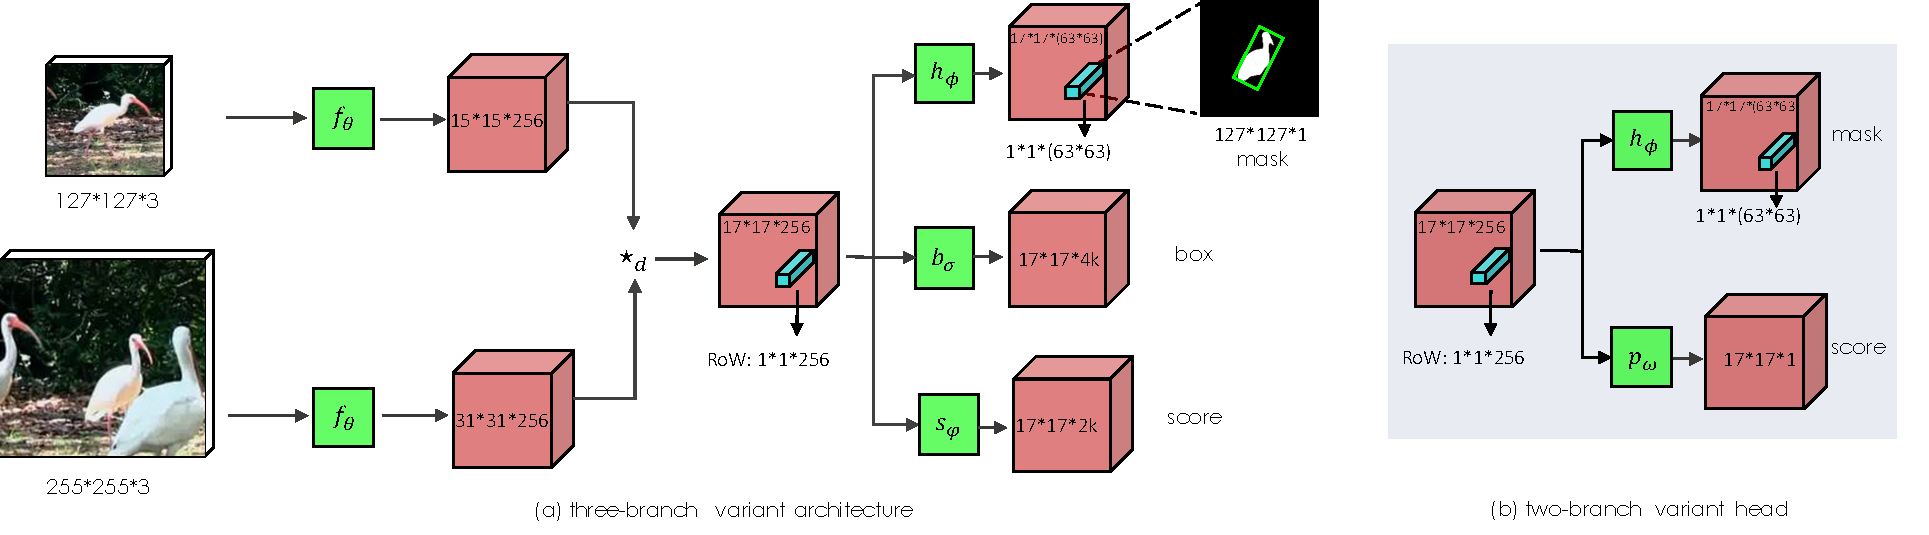
\includegraphics[width=1.0 \textwidth]{img/32branch.pdf}
\end{center}
\caption{Schematic illustration of SiamMask variants: (a) \textit{three-branch} architecture (full), (b) \textit{two-branch} architecture (head).  $\star_d$ denotes depth-wise cross correlation. For simplicity, upsampling layer and mask refinement module are omitted here and detailed in Appendix~\ref{sec:appendix_architecture}.}
\label{fig:schematic}
\vspace{-0.2cm}
\end{figure*}

\subsection{SiamMask}
\label{sec:siammask}
Unlike existing tracking methods that rely on low-fidelity object representations, we argue the importance of producing per-frame binary segmentation masks.
To this aim we show that, besides similarity scores and bounding box coordinates, it is possible for the RoW of a fully-convolutional Siamese network to also encode the information necessary to produce a pixel-wise binary mask.
This can be achieved by extending existing Siamese trackers with an extra branch and loss.

We predict $w{\times}h$ binary masks (one for each RoW) using a simple two-layers neural network $h_{\phi}$ with learnable parameters $\phi$.
Let $m_{n}$ denote the predicted mask corresponding to the $n$-th RoW,
\begin{equation}\label{eq:mask}
m_{n} = h_{\phi}(g_{\theta}^{n}(z,~x)).
\end{equation}
From Eq.~\ref{eq:mask} we can see that the mask prediction is a function of \emph{both} the image to segment $x$ and the target object in $z$.
In this way, $z$ can be used as a reference to guide the segmentation process:
given a different reference image, the network will produce a different segmentation mask for $x$.

\mypar{Loss function.}
During training, each RoW is labelled with a ground-truth binary label $y_{n} \in \{\pm 1\}$ and also associated with a pixel-wise ground-truth mask $c_n$ of size $w{\times}h$.
Let $c^{ij}_{n} \in \{\pm 1\}$ denote the label corresponding to pixel $(i,j)$ of the object mask in the $n$-th candidate RoW.
The loss function $\mathcal{L}_{mask}$ (Eq.~\ref{eq:loss}) for the mask prediction task is a binary logistic regression loss over all RoWs:

\begin{equation}\label{eq:loss}
		\mathcal{L}_{mask}(\theta,~\phi) =  \sum_{n} (\frac{1+y_{n}}{2wh}\sum_{ij} \log (1 + e^{-c^{ij}_{n}m_{n}^{ij}}
		)).
\end{equation}
Thus, the classification layer of $h_{\phi}$ consists of $w{\times}h$ classifiers, each indicating whether a given pixel belongs to the object in the candidate window or not.
Note that $\mathcal{L}_{mask}$ is considered only for positive RoWs (\ie with $y_{n}=1$).


\mypar{Mask representation.}
In contrast to semantic segmentation methods in the style of FCN~\cite{long2015fully} and Mask R-CNN~\cite{maskrcnn}, which maintain explicit spatial information throughout the network, our approach follows the spirit of~\cite{DeepMask,SharpMask} and generates masks starting from a flattened representation of the object.
In particular, in our case this representation corresponds to one of the ($17{\times}17$) RoWs produced by the depth-wise cross-correlation between $f_\theta(z)$ and $f_\theta(x)$.
Importantly, the network $h_\phi$ of the segmentation task is composed of two $1{\times}1$ convolutional layers, one with 256 and the other with $63^2$ channels (Figure~\ref{fig:schematic}).
This allows every pixel classifier to utilise information contained in the entire RoW and thus to have a complete view of its corresponding candidate window in $x$, which is critical to disambiguate between instances that look like the target (\eg last row of Figure~\ref{fig:davis16}), often referred to as distractors.
With the aim of producing a more accurate object mask, we follow the strategy of~\cite{SharpMask}, which merges low and high resolution features using multiple~\textit{refinement} modules made of upsampling layers and skip connections (see Appendix~\ref{sec:appendix_architecture}).

\mypar{Two variants.}
For our experiments, we augment the architectures of SiamFC~\cite{bertinetto2016fully} and SiamRPN~\cite{SiamRPN} with our segmentation branch and the loss $\mathcal{L}_{mask}$, obtaining what we call the \emph{two-branch} and \emph{three-branch} variants of SiamMask.
These respectively optimise the multi-task losses $\mathcal{L}_{2B}$ and $\mathcal{L}_{3B}$, defined as:
\begin{equation}
\label{eq:2b}
\mathcal{L}_{2B} = \lambda_{1} \cdot \mathcal{L}_{mask} + \lambda_{2} \cdot \mathcal{L}_{sim},
\end{equation}
\begin{equation}
\label{eq:3b}
\mathcal{L}_{3B} = \lambda_{1} \cdot \mathcal{L}_{mask} + \lambda_{2} \cdot \mathcal{L}_{score}+ \lambda_{3} \cdot \mathcal{L}_{box}.
\end{equation}
We refer the reader to~\cite[Section 2.2]{bertinetto2016fully} for $\mathcal{L}_{sim}$ and to~\cite[Section 3.2]{SiamRPN} for $\mathcal{L}_{box}$ and $\mathcal{L}_{score}$. 
For $\mathcal{L}_{3B}$, a RoW is considered positive ($y_{n} = 1$) if one of its anchor boxes has IOU with the ground-truth box of at least 0.6 and negative ($y_{n} = -1$) otherwise.
For $\mathcal{L}_{2B}$, we adopt the same strategy of~\cite{bertinetto2016fully} to define positive and negative samples.
We did not search over the hyperparameters of Eq.~\ref{eq:2b} and Eq.~\ref{eq:3b} and simply set $\lambda_1=32$ like in~\cite{DeepMask} and $\lambda_{2}=\lambda_{3}=1$.
The task-specific branches for the box and score outputs are constituted by two $1{\times}1$ convolutional layers.
Figure~\ref{fig:schematic} illustrates the two variants of SiamMask.


\mypar{Box generation.}
Note that, while VOS benchmarks require binary masks, typical tracking benchmarks such as VOT~\cite{kristan2016visual,VOT2018} require a bounding box as final representation of the target object.
We consider three different strategies to generate a bounding box from a binary mask (Figure~\ref{fig:bbox}):
(1) axis-aligned bounding rectangle (\emph{Min-max}), (2) rotated minimum bounding rectangle (\emph{MBR}) and (3) the optimisation strategy used for the automatic bounding box generation proposed in VOT-2016~\cite{kristan2016visual} (\emph{Opt}).
We empirically evaluate these alternatives in Section~\ref{sec:experiments} (Table~\ref{tab:iou}).

\begin{figure}[t]
\centering
\setlength{\tabcolsep}{0.25ex}

\begin{tabular}
{c cccc}
& 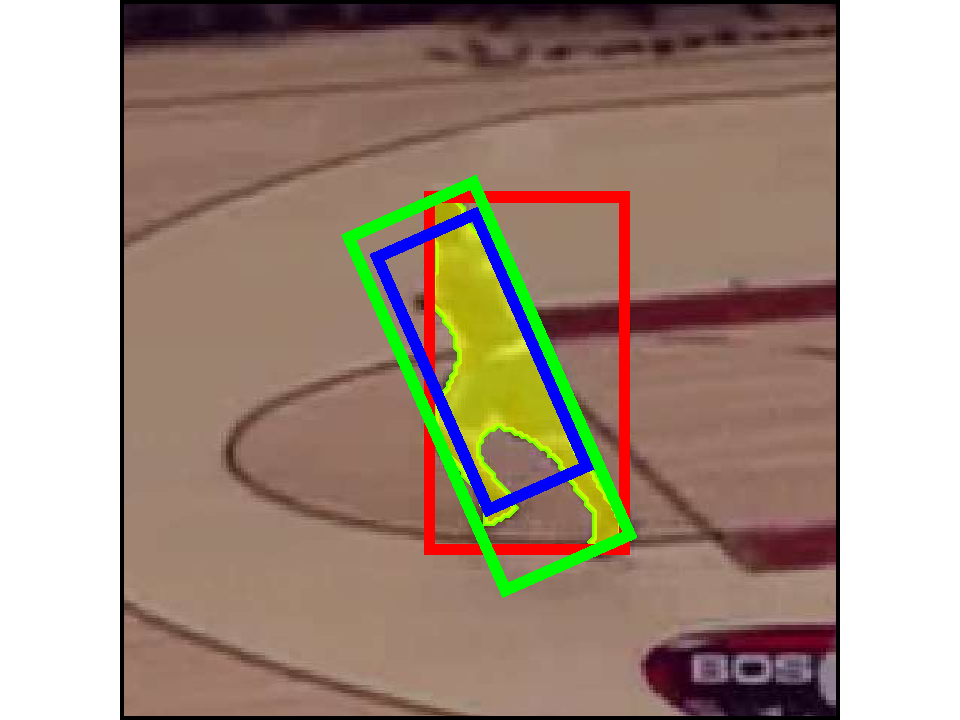
\includegraphics[trim={2cm 0cm 2cm 0cm},clip,width = 0.79in]{img/bbox/00435}
& 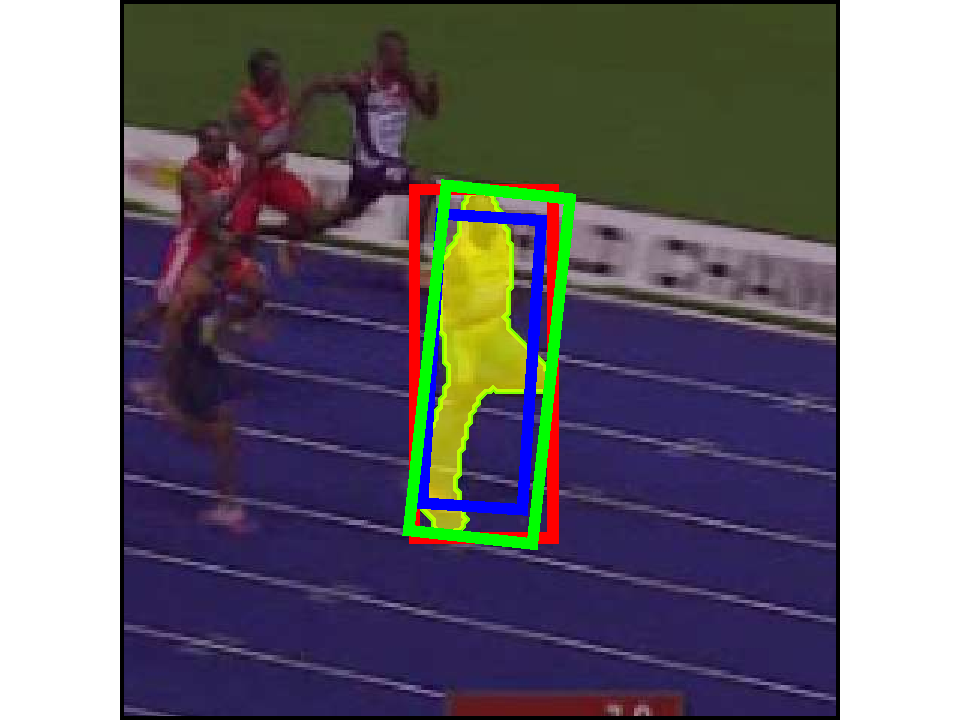
\includegraphics[trim={2cm 0cm 2cm 0cm},clip,width = 0.79in]{img/bbox/02411}
& 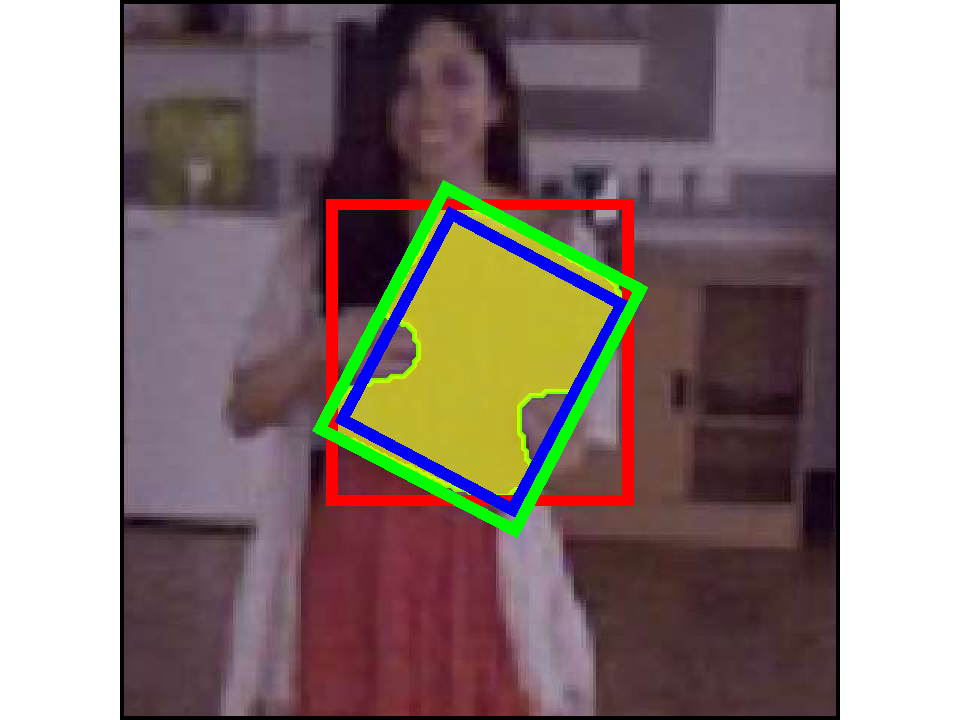
\includegraphics[trim={2cm 0cm 2cm 0cm},clip,width = 0.79in]{img/bbox/03046}
& 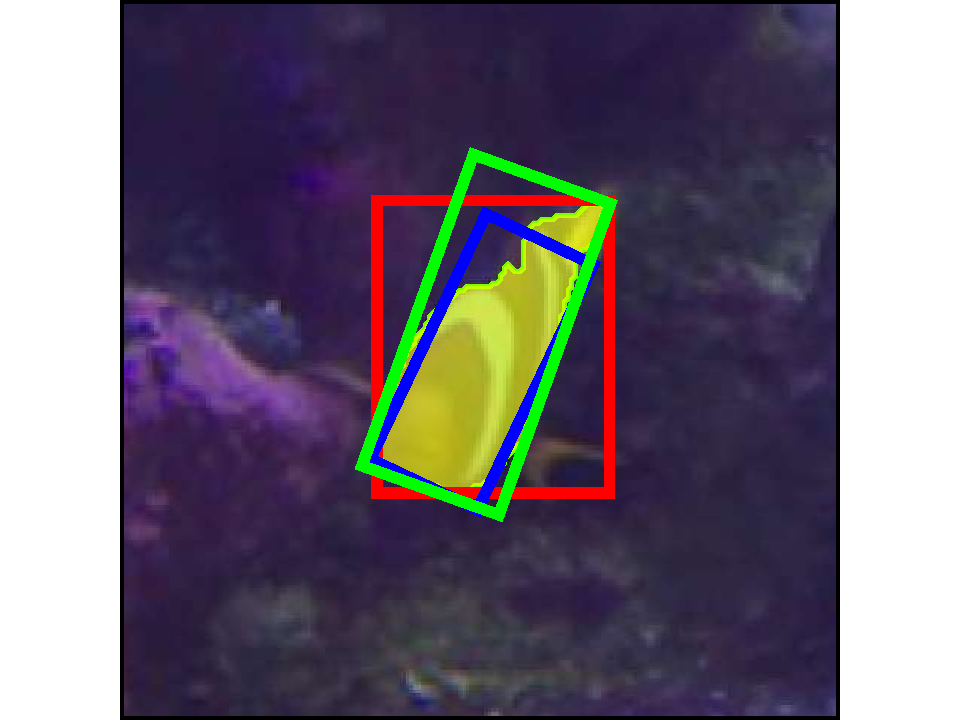
\includegraphics[trim={2cm 0cm 2cm 0cm},clip,width = 0.79in]{img/bbox/06761}
\\


\end{tabular}

\caption{
In order to generate a bounding box from a binary mask (in yellow), we experiment with three different methods.
\textit{Min-max}: the axis-aligned rectangle containing the object (red); \textit{MBR}: the minimum bounding rectangle (green); \textit{Opt}: the rectangle obtained via the optimisation strategy proposed in VOT-2016~\cite{kristan2016visual} (blue).}
\vspace{-1em}
\label{fig:bbox}
\end{figure}

\subsection{Implementation details}
\mypar{Network architecture.}
For both our variants, we use a ResNet-50~\cite{he2016deep} until the final convolutional layer of the \mbox{$4$-th} stage as our backbone $f_\theta$.
In order to obtain a high spatial resolution in deeper layers, we reduce the output stride to $8$ by using convolutions with stride 1.
Moreover, we increase the receptive field by using dilated convolutions~\cite{chen2018deeplab}.
In our model, we add to the shared backbone $f_{\theta}$ an unshared \emph{adjust} layer ($1{\times}1$ \textit{conv} with $256$ outputs). 
For simplicity, we omit it in Eq.~\ref{eq:cross}.
We describe the network architectures in more detail in Appendix~\ref{sec:appendix_architecture}.

\mypar{Training.}
Like SiamFC~\cite{bertinetto2016fully}, we use examplar and search image patches of $127{\times}127$ and $255{\times}255$ pixels respectively.
During training, we randomly jitter examplar and search patches.
Specifically, we consider random translations (up to $\pm 8$ pixels) and rescaling (of $2^{\pm 1/8}$ and $2^{\pm 1/4}$ for examplar and search respectively).

The network backbone is pre-trained on the \mbox{ImageNet-$1k$} classification task.
We use SGD with a first \emph{warmup} phase in which the learning rate increases linearly from $10^{-3}$ to $5{\times}10^{-3}$ for the first 5 epochs and then descreases logarithmically until $5{\times}10^{-4}$ for 15 more epochs.
We train all our models using COCO~\cite{lin2014microsoft}, ImageNet-VID~\cite{russakovsky2015imagenet} and YouTube-VOS~\cite{xu2018youtube}. 

\mypar{Inference.}
During tracking, SiamMask is simply evaluated once per frame, without any adaptation.
In both our variants, we select the output mask using the location attaining the maximum score in the classification branch.
Then, after having applied a per-pixel sigmoid, we binarise the output of the mask branch at the threshold of $0.5$.
In the \textit{two-branch} variant, for each video frame after the first one, we fit the output mask with the \emph{Min-max} box and use it as reference to crop the next frame search region.
Instead, in the \textit{three-branch} variant, we find more effective to exploit the highest-scoring output of the box branch as reference.

